\documentclass{report}

\usepackage{report_style}

\usepackage{eso-pic}


\graphicspath{{images/}}
%\usepackage{color}
\definecolor{bannercolor}{rgb}{0.3922,0.5843,0.9294}

\RequirePackage{geometry}
%\newgeometry{vmargin={25mm, 30mm}, hmargin={15mm,15mm}}   % set page margins

%\usepackage[svgnames]{xcolor}
%\usepackage{tikz}

\usepackage[absolute]{textpos}
\usepackage[]{rotating}

%\usepackage[]{titlesec} % to make titlepage work

\usepackage{graphicx} % load image
\usepackage{parskip} % adjust title/subtitle/etc

\usepackage{tocloft} % move down Contents
\setlength{\cftbeforesecskip}{5pt}

\definecolor{MediumBlue}{RGB}{38, 119, 193}

\titleformat{\chapter}[block]
%{\sffamily\LARGE}
{\color{white}\sffamily\bfseries\Large}
{} % chapter number usually
{0pt}
{\colorsectiona}

\titlespacing*{\chapter}{0pt}{\baselineskip}{\baselineskip}

\newcommand{\colorsectiona}[1]{%
% fboxsep: the distance between the frame and the content
	\colorbox{DarkBlue}{\parbox[c][20pt]{\dimexpr\textwidth-2\fboxsep}{\thechapter.~#1}}}

% overwrite chapter first page from plain to fancy in order to show header/footer
% https://tex.stackexchange.com/questions/117328/fancyhdr-does-not-apply-same-header-footer-on-chapter-and-non-chapter-pages
%\usepackage{etoolbox}
%\patchcmd{\chapter}{\thispagestyle{plain}}{\thispagestyle{fancy}}{}{}

\begin{document}


    \setlength{\TPHorizModule}{1mm}
    \setlength{\TPVertModule}{1mm}

    \begin{titlepage}
        \newgeometry{vmargin={30mm, 30mm}, hmargin={30mm,30mm}}
        \begin{textblock}{50}(-10,-10)
            \begin{color}{MediumBlue}
                \rule{3cm}{30cm} % width and length of the strip
            \end{color}
        \end{textblock}

        \begin{textblock}{20}(12,70) % x, y of upper left
            \begin{rotate}{90}
            {\huge\bfseries \textcolor{white}{Programming}}
            \end{rotate}
        \end{textblock}

        \begin{textblock}{150}(30,30) %, length, x-coord, y-coord of upper left corner
            
\includegraphics[height=20mm]{images/panda}\medskip

            {\huge\bfseries Application Design and Architecture }\medskip

            {\Large\bfseries How to Write Reusable and Maintainable Code }\medskip

            {\large\today}\vspace{10mm}

            {\large\bfseries Firstname Lastname}
        \end{textblock}

        \setlength{\cftbeforetoctitleskip}{300pt} % move content down by this much
        \setlength{\cftaftertoctitleskip}{20pt}
        \tableofcontents

        \thispagestyle{empty} % remove page number
	\end{titlepage}

    %\newpage

    \chapter{Analysis Report}
    \thispagestyle{fancy} % in order to show header/footer

    This is a tool.

	\section{Acornyms}

	Lorem ipsum dolor sit amet, consectetur adipiscing elit. Donec nec fermentum augue. Integer id neque sit amet augue lacinia fringilla. Donec leo ipsum, dapibus vel orci et, viverra viverra sem. Morbi maximus neque ipsum, in vulputate libero porta a. Interdum et malesuada fames ac ante ipsum primis in faucibus. Nulla at libero arcu.


	\begin{figure}[htb]
		\centering
		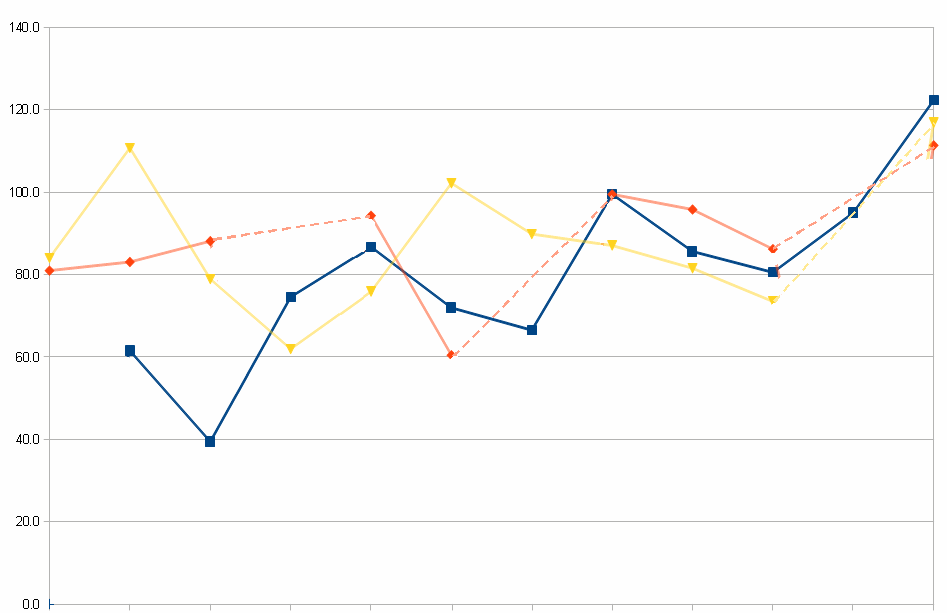
\includegraphics[width=1\textwidth]{figure1}
		\centering
		\textcolor{Orange}{\textbf{\caption{Figure Description}}}\label{fig:1}
	\end{figure}

    The chart is nice, imported.

	\section{Excel}

	In pretium enim dui, quis ornare odio varius et. Nulla facilisi. Nunc tristique tortor
	at urna vehicula, elementum bibendum tortor hendrerit. Ut eu risus nisi. Vestibulum nunc
	lorem, tristique sed ultrices nec, porta et ligula. Nam facilisis felis a congue auctor.
	Fusce id odio in libero blandit cursus nec nec arcu. Nulla eu ultricies massa, id dapibus nisi. Donec tellus urna, maximus nec semper id, consectetur eu mi. Vestibulum elit eros, porta ac eros a, mattis pulvinar magna. Nulla pellentesque dapibus leo molestie varius. Duis ut rutrum urna, at condimentum dui. Sed orci magna, faucibus nec quam et, malesuada ultrices velit. Nam a lorem a massa facilisis rutrum eget id nunc. Morbi aliquet felis et tincidunt scelerisque.

    % https://tex.stackexchange.com/questions/24066/start-new-chapter-on-same-page
    % keep chapter on the same page, rather than a new page
    \begingroup
    \let\clearpage\relax
    \chapter{Next Tool}
    \endgroup

    \thispagestyle{fancy} % in order to show header/footer
%    \chapter{Next Tool}
%    \thispagestyle{fancy} % in order to show header/footer

    This is check header
    \section{Python}
	In pretium enim dui, quis ornare odio varius et. Nulla facilisi. Nunc tristique tortor at urna vehicula, elementum bibendum tortor hendrerit. Ut eu risus nisi. Vestibulum nunc lorem, tristique sed ultrices nec, porta et ligula. Nam facilisis felis a congue auctor. Fusce id odio in libero blandit cursus nec nec arcu. Nulla eu ultricies massa, id dapibus nisi. Donec tellus urna, maximus nec semper id, consectetur eu mi. Vestibulum elit eros, porta ac eros a, mattis pulvinar magna. Nulla pellentesque dapibus leo molestie varius. Duis ut rutrum urna, at condimentum dui. Sed orci magna, faucibus nec quam et, malesuada ultrices velit. Nam a lorem a massa facilisis rutrum eget id nunc. Morbi aliquet felis et tincidunt scelerisque.

    \section{Scala}
	In pretium enim dui, quis ornare odio varius et. Nulla facilisi. Nunc tristique tortor at urna vehicula, elementum bibendum tortor hendrerit. Ut eu risus nisi. Vestibulum nunc lorem, tristique sed ultrices nec, porta et ligula. Nam facilisis felis a congue auctor. Fusce id odio in libero blandit cursus nec nec arcu. Nulla eu ultricies massa, id dapibus nisi. Donec tellus urna, maximus nec semper id, consectetur eu mi. Vestibulum elit eros, porta ac eros a, mattis pulvinar magna. Nulla pellentesque dapibus leo molestie varius. Duis ut rutrum urna, at condimentum dui. Sed orci magna, faucibus nec quam et, malesuada ultrices velit. Nam a lorem a massa facilisis rutrum eget id nunc. Morbi aliquet felis et tincidunt scelerisque.

\end{document}
